\section{Prior Work Completed\label{introduction:priorWork}}

This project idea of an improved lumpectomy tumor bed marking method was first proposed by the Division Chief for Oncoplastic Surgery at The Ohio State University Comprehensive Cancer Center (OSUCCC), Dr. Roman Skoracki~\cite{RefWorks:RefID:372-krakovskytumor},~\cite{RefWorks:RefID:371-bakhtardesign}.

This project was then adopted bya mechanical engineering senior capstone in 2022 (\hl{Check this date}). It has since been further explored by Adrian Bakhtar, Isaac Einstein, and Zuhaib Jama. The general contributions of each group are summarized below in Table~\ref{tab:introduction:priorWorkCompletedOverview}.

\begin{table}[H]
        \centering
        \caption{Summary of Prior Team and Researcher Contributions}
        \label{tab:introduction:priorWorkCompletedOverview}
        \begin{tabularx}{\textwidth}{>{\raggedright\arraybackslash}p{3cm} X >{\raggedright\arraybackslash}p{3cm}}
                \toprule
                \textbf{Team/Researcher}                                       & \textbf{General Contribution(s)} & \textbf{Time Working on Project} \\
                \midrule
                Senior Capstone Group~\cite{RefWorks:RefID:372-krakovskytumor} &
                - Identified initial pain points and opportunity \newline
                - Evaluated various end-product concepts \newline
                - Selected ideal form factor and developed initial device prototype
                                                                               & 2022                                                                \\
                \addlinespace
                Adrian Bakhtar~\cite{RefWorks:RefID:371-bakhtardesign}         &
                - Continued work started by senior capstone team \newline
                - Worked with stakeholders to refine device design \newline
                - Optimized device geometry, printability, and adhesive capabilities \newline
                - Defended master's thesis and is continuing research through a PhD
                                                                               & 2022 -- Present                                                     \\
                \addlinespace
                Zuhaib Jama~\cite{RefWorks:RefID:384-jamacomputational}        &
                - Evaluated potential stresses experienced by the device via FEM \newline
                - Presented findings at research poster symposium
                                                                               & 2024                                                                \\
                \addlinespace
                Isaac Einstein~\cite{RefWorks:RefID:370-einsteinisaac}         &
                - Evaluated material properties of device base material \newline
                - Presented findings through a research poster symposium and undergraduate thesis
                                                                               & 2023 -- 2024                                                        \\
                \bottomrule
        \end{tabularx}
\end{table}

\subsection{Senior Capstone Work\label{sec:introduction:priorWork:seniorCapstone}}

\subsubsection{Device Requirements\label{sec:introduction:priorWork:seniorCapstone:deviceRequirements}}
Working alongside the OSUCCC including surgeons, radiation oncologists, and dosimetrists, the senior capstone team developed target functional requirements for the device. This is outlined below in Table~\ref{tab:introduction:priorWork:seniorCapstone:targetSpecifications}.

\begin{table}[H]
        \centering
        \caption{Initial Device Target Specifications~\cite{RefWorks:RefID:372-krakovskytumor},~\cite{RefWorks:RefID:371-bakhtardesign}}
        \label{tab:introduction:priorWork:seniorCapstone:targetSpecifications}
        \begin{tabularx}{\textwidth}{
                >{\centering\arraybackslash}p{1.2cm}
                >{\raggedright\arraybackslash}p{3.5cm}
                X
                }
                \toprule
                \textbf{Weight} & \textbf{Specification} & \textbf{Requirement} \\
                \midrule
                1               & Biocompatibility       &
                Follows ISO 10993 \newline
                • Twenty-part protocol FDA testing process                      \\
                \addlinespace
                2               & Sterilizable           &
                Follows ISO 11135 \newline
                • Sterilization of health-care products (Ethylene oxide) \newline
                Packaging follows ISO 11607 \newline
                • Packaging for sterilized material                             \\
                \addlinespace
                3               & Implantation speed     &
                < 3 minutes                                                     \\
                \addlinespace
                4               & Radiodensity           &
                > 0 HU and < 3000 HU (Hounsfield Units)                         \\
                \addlinespace
                5               & Longevity              &
                6 weeks -- 12 months                                            \\
                \addlinespace
                6               & Mechanical Properties  &
                812 -- 4500 kg/m\textsuperscript{3}                             \\
                \addlinespace
                7               & Size/Area              &
                2 -- 7 cm in diameter \newline
                10 -- 150 cm\textsuperscript{2}                                 \\
                \addlinespace
                8               & Cost                   &
                < \$1250                                                        \\
                \bottomrule
        \end{tabularx}
\end{table}

Because the device would eventually be implanted in human patients, biocompatibility and sterilization were given the highest importance. Implantation speed was next based on surgeon feedback~\cite{RefWorks:RefID:372-krakovskytumor}.

It was believed the chances of device adoption by surgeons would decrease if implantation speed was significant~\cite{RefWorks:RefID:372-krakovskytumor}.

Discussions with dosimetrists led the group to select a target Hounsfield Units (HU) of less than 3,000 HU to reduce radiation reflection and provide adequate contrast from breast tissue~\cite{RefWorks:RefID:372-krakovskytumor}.

The longevity of the device was estimated through conversations with OSUCCC based on the range of lumpectomy procedure timelines~\cite{RefWorks:RefID:372-krakovskytumor}.

The mechanical properties were selected to mirror breast tissue based on additional team research~\cite{RefWorks:RefID:372-krakovskytumor}.

Lastly, the size and cost of the device were selected based on research into existing competitor devices~\cite{RefWorks:RefID:372-krakovskytumor}.

\subsubsection{Initial Prototype Development\label{sec:introduction:priorWork:seniorCapstone:initialPrototypeDevelopment}}

\paragraph*{Material Selection\label{sec:introduction:priorWork:seniorCapstone:initialPrototypeDevelopment:materialSelection}}
To adhere with the mechanical properties and biodegradable needs of the device, the capstone team selected Poly(l-lactide-co-$\varepsilon$-caprolactone) (PLCL) as the base material. This is a biodegradable and biocompatible material with an adjustable degredation timeline and mechanical properties. It is composed of two co-polymers: Polylactic acid (PLA) and Polycaprolactone (PCL). The radiopaque agent selected was barium sulfate (BaSO4) based on its extensive clinical trials and current use in digestive marking~\cite{RefWorks:RefID:372-krakovskytumor}.

\paragraph*{Device Form Factor\label{sec:introduction:priorWork:seniorCapstone:initialPrototypeDevelopment:formFactor}}
As shown in Figure~\ref{fig:introduction:initialCapstonePrototype}, the capstone team designed the device in a hemispherical and collapsible form factor. The team created the prototype through melting base materials into a premade mold~\cite{RefWorks:RefID:372-krakovskytumor}.

\paragraph*{Imaging Testing\label{sec:introduction:priorWork:seniorCapstone:initialPrototypeDevelopment:imaginTesting}}

Imaging capabilities and radiopacity of the initial prototype was evaluated by the capstone team to evaluate the desired amount of barium sulfate. This initial testing resulted in excessively bright samples, which illustrated the need to minimal barium sulfate addition~\cite{RefWorks:RefID:372-krakovskytumor}. The capstone team's imaging testing is shown below in Figure~\ref{fig:introduction:capstoneImagingTesting}.

\begin{figure}[h!]
        \centering
        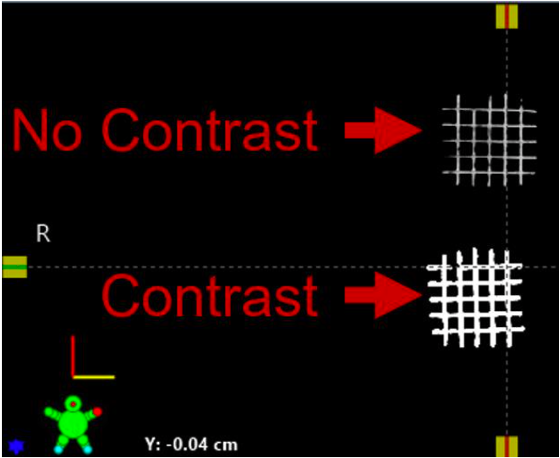
\includegraphics[width=0.8\textwidth]{../figs/introduction/capstone_imaging_testing.png}
        \caption{Initial imaging results from senior capstone team~\cite{RefWorks:RefID:372-krakovskytumor}.}
        \label{fig:introduction:capstoneImagingTesting}
\end{figure}

\subsection{Additional Research Team Work\label{sec:introduction:priorWork:otherTeamWork}}

\subsubsection{Design of Device\label{sec:introduction:priorWork:otherTeamWork:deviceDesign}}
% a.	Device geometry
% b.	Surface texture
% c.	Friction testing

\subsubsection{Material Evaluation\label{sec:introduction:priorWork:otherTeamWork:materialEval}}
% a.	Biodegradability testing

\subsubsection{3D Printing Work\label{sec:introduction:priorWork:otherTeamWork:3dPrinting}}
% a.	Optimizing PLCL printing parameters
% b.	Layer shape

\subsubsection{Customer Discovery\label{sec:introduction:priorWork:otherTeamWork:customerDiscovery}}
% a.	I-Corps
% i.	Led to thin sheet instead of patient-specific shape

\subsection{Undergraduate Thesis\label{sec:introduction:priorWork:undergradThesis}}

\subsubsection{Felfil Extrusion Work\label{sec:introduction:priorWork:undergradThesis:felfil}}
% Trying to extrude a powder unsuccessfully

\subsubsection{Mechanical Testing of Lattice PLCL Filaments\label{sec:introduction:priorWork:undergradThesis:mechTesting}}
% a. Tensile Strength
% b. Flexural Modulus
